\documentclass[cn]{homework}

\title{作业5}

\DeclareMathOperator{\var}{Var}
\DeclareMathOperator{\E}{E}
\begin{document}
    \maketitle

    \problem
    \begin{proof}
        为记号的简便性,我们记
        \[\E(Y|X)=Y'\]
        考虑
        \[\begin{aligned}
            \mathrm{MSE}
            &=\E(Y-g(X))^2\\
            &=\E(Y-Y'+Y'-g(X))^2\\
            &=\E(Y-Y')^2-2\E((Y-Y')(Y'-g(X)))+\E(Y'-g(X))^2\\
        \end{aligned}\]
        而中间项
        \[\begin{aligned}
            \E((Y-Y')(Y'-g(X)))&=\E(Y(Y'-g(X)))-\E(Y'(Y'-g(X)))
        \end{aligned}\]
        注意到$Y'-g(X)$是$\sigma(X)$可测的,于是
        \[\begin{aligned}
            \E(Y'(Y'-g(X)))&=\E((Y'-g(X))\E(Y|X))\\
            &=\E\Big(\E\big(Y(Y'-g(X))|X\big)\Big)\\
            &=\E(Y(Y'-g(X)))
        \end{aligned}\]
        因此中间项
        \[\E((Y-Y')(Y'-g(X)))=0\]
        故
        \[\begin{aligned}
           \mathrm{MSE}&=\E(Y-Y')^2+\E(Y'-g(X))^2\\
           &=\E(Y-\E(Y|X))^2+\E(g(X)-\E(Y|X))^2
        \end{aligned}\]
        显然,仅在
        \[g(X)=\E(Y|X)\quad\mathrm{a.e.}\]
        时能取得最小值
        \[\E(Y-\E(Y|X))^2\]
    \end{proof}

    \problem
    \begin{subproblem}[(\alph*)]
        \item
        题中ARMA模型可以写为
        \[(1-\phi B)Y_t=(1-\theta B)Z_t\]
        考虑其传递模式有
        \[\begin{aligned}
            \frac{1-\theta B}{1-\phi B}
            &=(1-\theta B)\sum_{i=0}^\infty(\phi B)^i\\
            &=1+(\phi-\theta)\sum_{i=1}^\infty\phi^{i-1}B^i\\
        \end{aligned}\]
        因此有Green函数
        \begin{equation}
            \label{eq:p2 Green}
            G_i=\begin{cases}
            1,&i=0\\
            (\phi-\theta)\phi^{i-1},&i>0
            \end{cases}\quad i=0,1,2,\ldots
        \end{equation}

        考虑到$\hat Y_m(s)$是$Z_m,Z_{m-1},\ldots$的线性函数,
        不妨设
        \[\hat Y_m(s)=\sum_{i=0}^\infty W_iZ_{m-i}\]
        而真实值
        \[Y_{m+s}=\sum_{i=0}^\infty G_iZ_{m+s-i}\]
        则误差
        \[\begin{aligned}
           e_m(s)&=Y_{m+s}-\hat Y_m(s)\\ 
           &=\sum_{i=0}^{s-1}G_iZ_{m+s-i}
             +\sum_{i=s}^\infty G_iZ_{m+s-i}
             -\sum_{i=0}^\infty W_iZ_{m-i}\\
           &=\sum_{i=0}^{s-1}G_iZ_{m+s-i}
             +\sum_{i=0}^\infty (G_{s+i}-W_i)Z_{m-i}
        \end{aligned}\]
        其方差为
        \[\begin{aligned}
            \var(e_m(s))&=\var\left(\sum_{i=0}^{s-1}G_iZ_{m+s-i}\right)
            +\var\left(\sum_{i=0}^\infty (G_{s+i}-W_i)Z_{m-i}\right)\\
            &=\sigma_Z^2\sum_{i=0}^{s-1}G_i^2
              +\var\left(\sum_{i=0}^\infty (G_{s+i}-W_i)Z_{m-i}\right)\\
        \end{aligned}\]
        其中$\sigma_Z^2$为白噪声的方差。
        显然,当
        \[W_i=G_{s+i},i=0,1,2,\ldots\]
        时可满足最小方差原则,
        此时方差为
        \begin{equation}
            \label{eq:p2 variance}
            \var(e_m(s))=\sigma_Z^2\sum_{i=0}^{s-1}G_i^2
        \end{equation}
        于是
        \[\hat Y_m(s)=\sum_{i=0}^\infty G_{s+i}Z_{m-i}\]
        其中$G_{s+i}$由\cref{eq:p2 Green}决定。

        \item
        由于模型平稳,因此有$|\phi|<1$,故对于任意$i\in\mathbb N$
        \[G_{s+i}\to 0\quad(s\to\infty)\]
        于是
        \[\hat Y_m(s)\to 0\quad(s\to\infty)\]
        即预测将趋于0。

        \item
        由\cref{eq:p2 variance}知
        \[\begin{aligned}
            \var(e_m(s))
            &=\left(1+(\phi-\theta)^2\sum_{i=1}^{s-1}\phi^{2i-2}\right)\sigma_Z^2\\
            &\to\left(1+\frac{(\phi-\theta)^2}{1-\phi^2}\right)\sigma_Z^2
             \quad(s\to\infty)
        \end{aligned}\]
        即方差将趋于
        \[\left(1+\frac{(\phi-\theta)^2}{1-\phi^2}\right)\sigma_Z^2\]
    \end{subproblem}

    \problem
    \begin{subproblem}[(\alph*)]
        \item
        首先对数据进行差分运算,并进行平稳性的判断,可以看到
        (\cref{fig:acf}),
        经过1阶差分后,数据可以判定是平稳的,2阶差分并没出现更
        明显的平稳性,于是判定$d=1$。

        \begin{figure}[h]
            \centering
            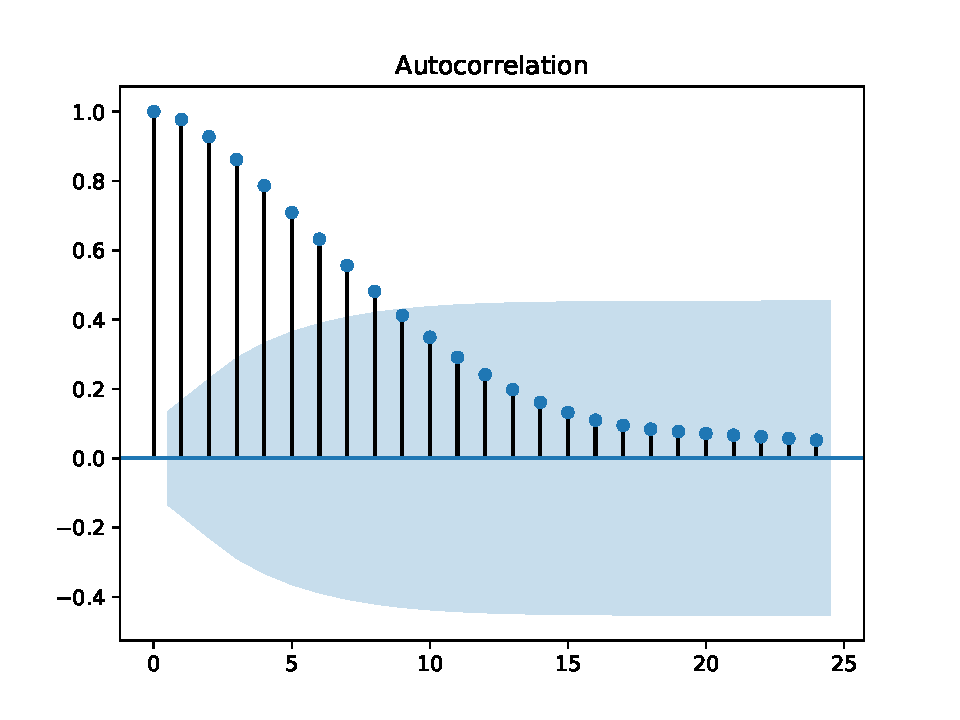
\includegraphics[width=0.32\linewidth]{acf-d0}
            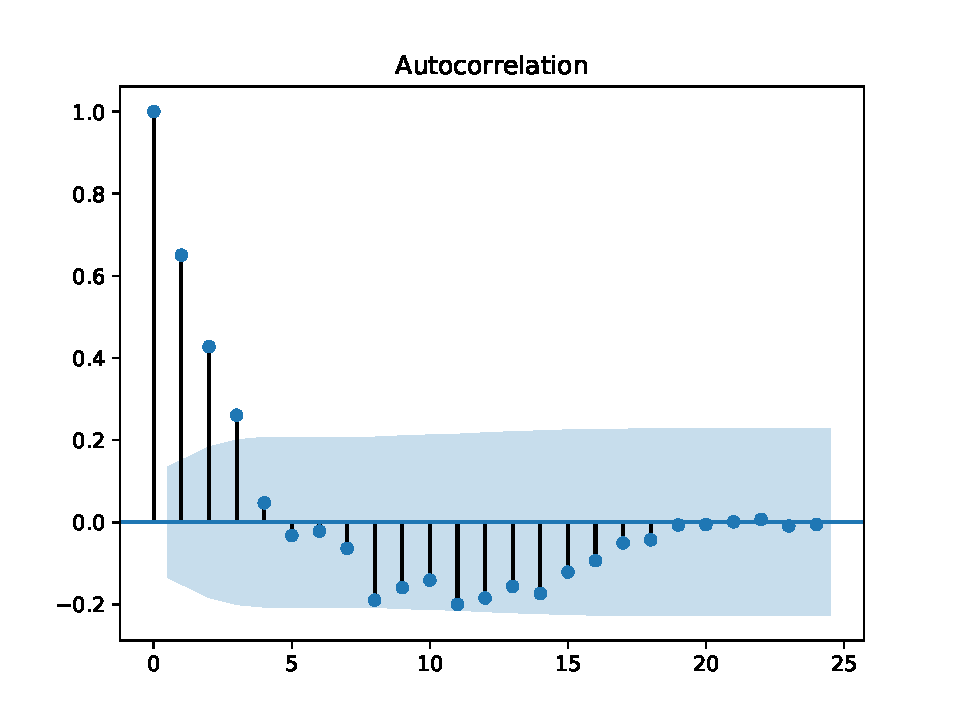
\includegraphics[width=0.32\linewidth]{acf-d1}
            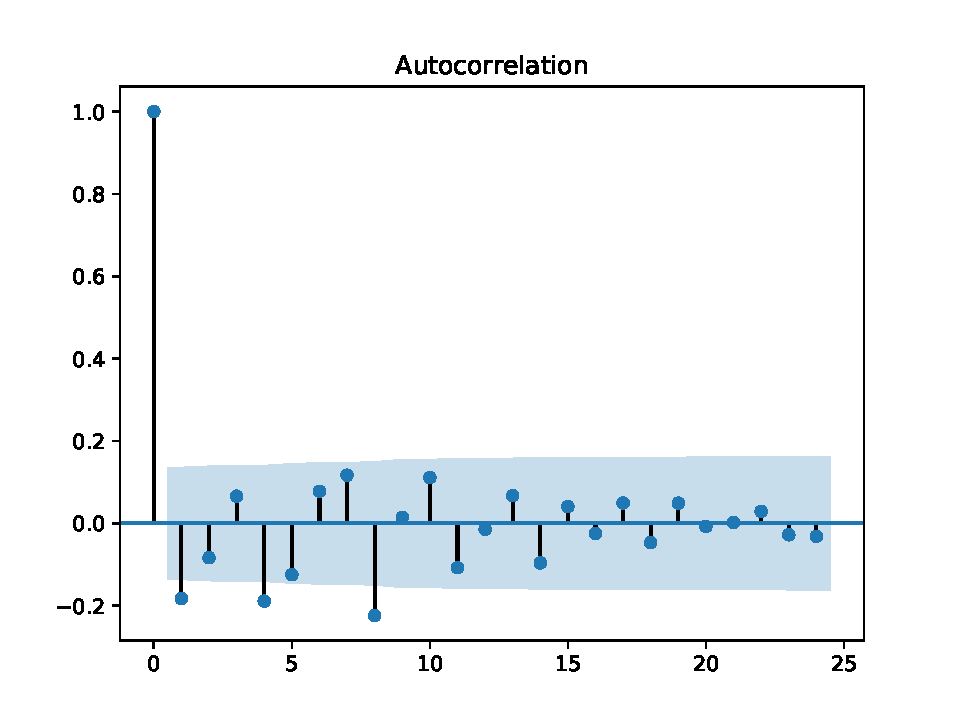
\includegraphics[width=0.32\linewidth]{acf-d2}
            \caption{不同阶数差分下的ACF}
            \label{fig:acf}
        \end{figure}

        \begin{marginfigure}
            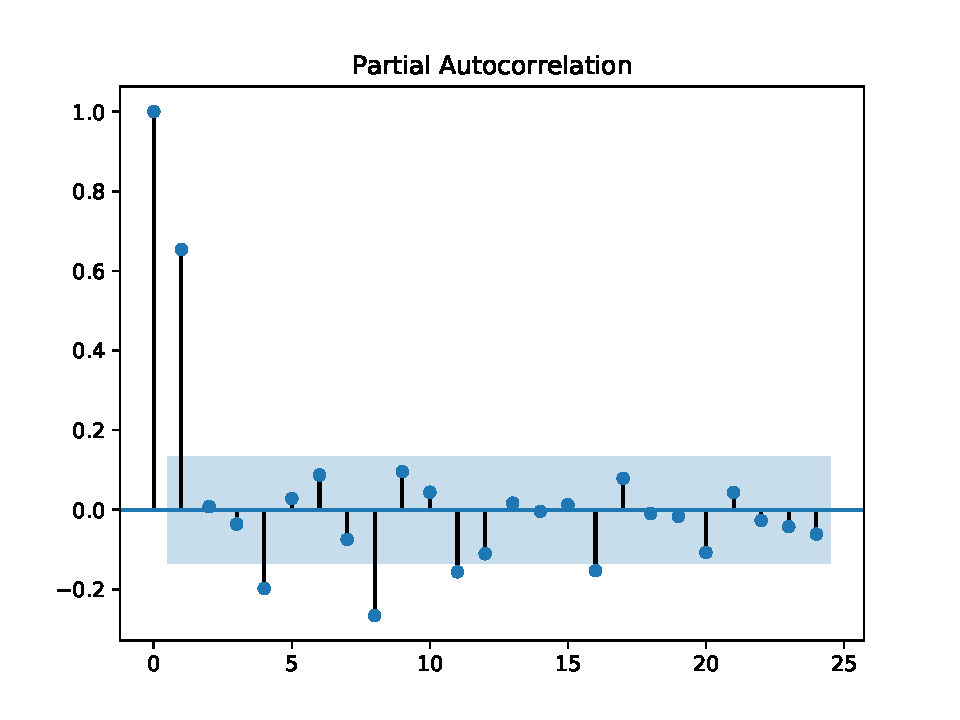
\includegraphics[width=0.9\textwidth]{pacf}
            \caption{PACF}
            \label{fig:pacf}
        \end{marginfigure}

        从ACF上能够看出,1阶差分后的序列差不多具有3阶截尾性,
        这是MA模型的典型特征,同时绘制PACF如\cref{fig:pacf}。
        具有1阶截尾性这是AR(1)的特征,于是我们可以考虑模型
        ARIMA(1,1,3)或者ARIMA(1,1,4)。

        经过拟合发现,ARIMA(1,1,3)的AIC与BIC稍大于ARIMA(1,1,4),
        但是差距并不是很明显(\cref{tab:AIC BIC}),
        以简单起见的原则,我们选用ARIMA(1,1,3)。

        \begin{margintable}
            \centering
            \begin{tabular}{ccc}
                \toprule
                模型 & AIC & BIC\\
                \midrule
                ARIMA(1,1,3) & -770.619& -750.508\\ 
                ARIMA(1,1,4) & -774.499 & -751.036\\
                \bottomrule
            \end{tabular}
            \caption{AIC与BIC}
            \label{tab:AIC BIC}
        \end{margintable}

        通过对模型进行估计,我们可以得到估计的模型方程为
        \[\Delta X_t+0.005\Delta X_{t-1}=0.0018+\epsilon_t-0.6356\epsilon_{t-1}
        -0.5663\epsilon_{t-2}-0.4986\epsilon_{t-3}\]

        同时对残差进行白噪声检验,可以得到$m=6,12$时的Q统计量
        (\cref{tab:residual test}),其$p$值是显著大于0.05的,
        因此可以认为通过了检验,残差项是白噪声。

        \begin{margintable}
            \centering
            \begin{tabular}{ccc}
                \toprule
                $m$ & $Q$ & $p$ \\
                \midrule
                6 & 4.3963 & 0.6232\\
                12 & 21.5272 & 0.0631\\
                \bottomrule
            \end{tabular}
            \caption{ARMIA(1,1,3)残差检验}
            \label{tab:residual test}
        \end{margintable}

        \begin{marginfigure}
            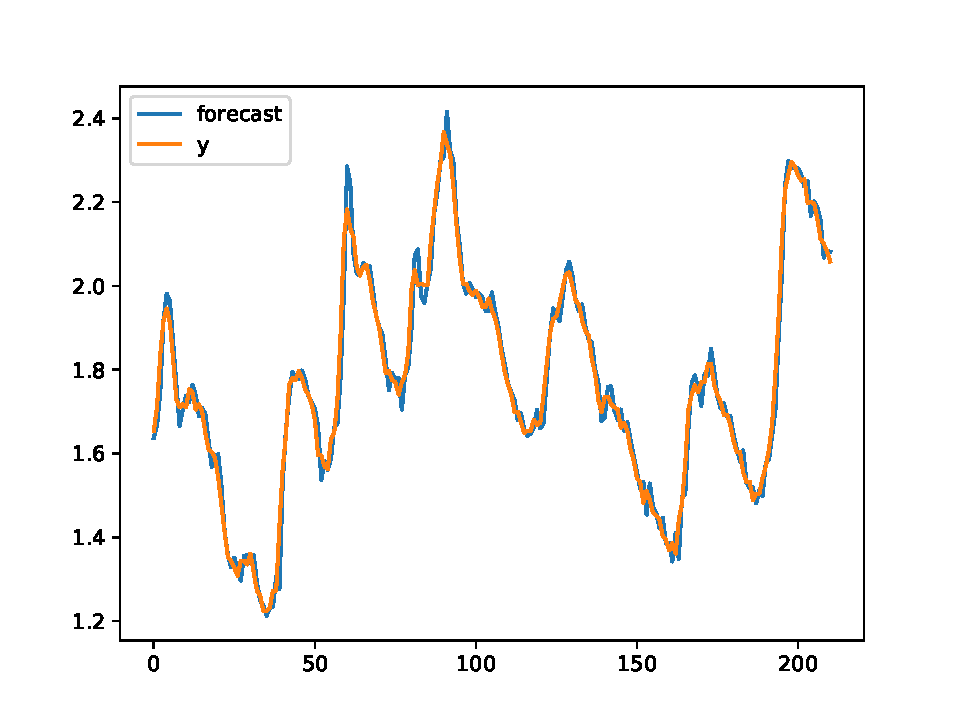
\includegraphics[width=0.9\textwidth]{real-prediction}
            \caption{真实值与预测值}
            \label{fig:residual}
        \end{marginfigure}
        
        \item
        如图
        \begin{table}[h]
            \centering
            \begin{tabular}{cccc}
                \toprule
                季度 & 实际值 & 预测值 & 误差\\
                \midrule
                2011Q1 & 2.19722 & 2.25107 & -0.05385\\
                2011Q2 & 2.20055 & 2.16733 & 0.03322\\
                2011Q3 & 2.19722 & 2.20148 & -0.00426\\
                2011Q4 & 2.15987 & 2.18824 & -0.02838\\
                2012Q1 & 2.11263 & 2.15776 & -0.04513\\
                2012Q2 & 2.10047 & 2.06754 & 0.03293\\
                2012Q3 & 2.08318 & 2.08346 & -0.00027\\
                2012Q4 & 2.05796 & 2.08093 & -0.02296\\
                \bottomrule
            \end{tabular}
        \end{table}
        \begin{figure}
            \centering
            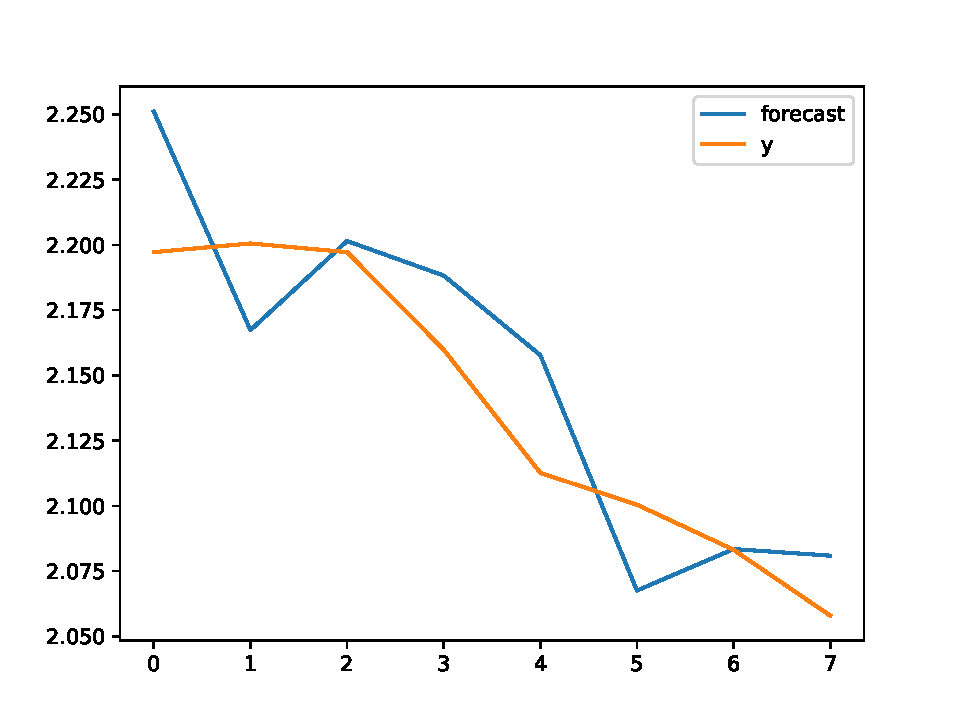
\includegraphics[width=0.8\linewidth]{tail-prediction}
        \end{figure}
    \end{subproblem}

    \newpage
    \appendix
    \section{Python代码}
    \lstinputlisting[language=Python]{main.py}
\end{document}